\subsection{Fehleranalyse}
Im Folgenden wollen wir auf mögliche Fehlerquellen eingehen und die Einflüsse derer
auf unsere Messungen erläutern:
\paragraph{Die durch die Spitzenherstellung} hervorgerufenen Fehlerspektren sind für 
den Großteil der Störungen in unseren Aufnahmen verantwortlich, da jene nach der Herstellung
einer geeigneten Spitze eliminiert waren, namentlich
\begin{itemize}
        \item Horizontale Schlieren und Streifen bis auf Pixelgröße. Dafür gibt 
            es behelfsweise die Möglichkeit, die Pixel eines lokalen, vertikalen Medians
            zu filtern und zu normalisieren; dieser Filter kann mit der Software Gwyddion
            angewandt werden.

        \item unkorreliertes Rauschen: Bei unkorreliertem Rauschen, das beispielsweise durch
            eine inhomogene, raue Spitze verursacht wird, kann letztere Methode zu keinem
            Ergebnis führen. In diesem Fall ist es zweckmäßig, die Periodizität, welche
            durch Korrelationen entsteht, mit der Autokorrelationstransformation zu verstärken
            und somit das unkorrelierte Rauschen herauszufiltern.
        \item mehrere Spitzen führen zu Geisterbildern. Diese Geisterbilder müssen qualitativ
            beurteilt werden und durch eventualle Filter eliminiert werden. In unserem
            Fall war es allerdings nicht möglich, Geisterbilder auf eine solche Weise
            zu lokalisieren, als dass wir sie hätten eliminieren können.
\end{itemize}
\paragraph{Die Schwingungseinflüsse} auf die Aufnahmen sind unter anderem in dünnen Linien
und Streifen erkennbar. Die Apperatur ist nicht perfekt Schwingungsgedämpft, nur dadurch
ist zu erklären, dass in manchen Aufnahmen nach einer gewissen Abrasterungszeit auf einmal
die Qualität deutlich schlechter wird (so wurden keine anderen Paramter des Systems geändert).
Allerdings ist es fraglich, ob die zur Verfügung stehende Dämpfungsbox einen Einfluss
auf diesen Störfaktor ausüben kann. 
\paragraph{Die Diskontinuität der Tunnelstromstärke} in einigen unserer Aufnahmen hat den
offensichtlichen Effekt auf die gemessene Topographie der Probe, dass die Strukturen nicht
abbildungstreu wiedergegeben werden, siehe Abbildung~\ref{fig:fehler1}. 

\begin{figure}[h]
    \begin{subfigure}[b]{\picwidth}
    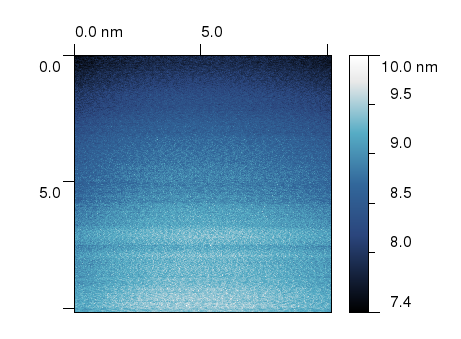
\includegraphics[width=\textwidth]{pics/fehler1a}
    \end{subfigure}\qquad
    \begin{subfigure}[b]{\picwidth}
        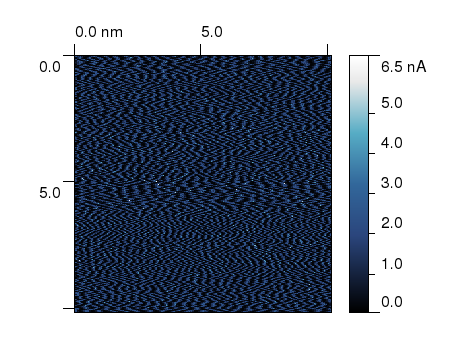
\includegraphics[width=\textwidth]{pics/fehler1b}
    \end{subfigure}
    \caption{Links: Aufnahme der Topographie, rechts: Aufnahme des Tunnelstroms.
    Offensichtlich war die Regelung nicht imstande, den Tunnelstrom konstant zu halten. 
    Somit konnte die Periodizität der Probe nicht auf in der Topographie visualisiert werden,
    da sie durch die Vorwegnahme des nicht konstanten Tunnelstroms marginalisiert wurde.}
    \label{fig:fehler1}
\end{figure}

Eine Lösung für diese Problematik bietet die Modifizierung der Parameter der Regelung. 
Einerseits ist es möglich, die Parameter des PID-Reglers zu modifizieren, dafür
ist eine fundierte Auseinandersetzung mit der Regelungstechnik des PID-Reglers nötig.
Ein unmittelbarer Paramter ist der ``Integral Gain'', welcher zur Kompensation eben dieses
Effekts dient, da er den Paramter des I-Gliedes darstellt,
und der ``Proportional Gain'' des P-Gliedes. Beide beeinflussen die Änderungsgeschwindigkeit
der Anpassung. Ein jeweils kleiner Wert führt somit eher zu einer trägeren Anpassung
der Spitze, während ein höherer Wert gegenteilig wirkt. Wird der Wert also zu klein gewählt,
ist keine Topographie mehr erkennbar. Wir waren mit der Einstellung dieses Werts vorsichtig,
da bei falscher Einstellung des Wertes auch eine Kollision der Spitze mit der Probe möglich wird.
Andererseits ist es möglich, die Rastergeschwindigkeit des RTMs so zu verringern, dass der
Regler genug Zeit für die Rückregelung des Tunnelstroms aufbringt; diese Maßnahme haben wir 
getroffen und konnten so die Qualität unserer Aufnahmen deutlich verbessern.
\paragraph{Ein Gradient in der Topographie} führte in vielen Aufnahmen
dazu, dass die periodischen Strukturen dadurch unterdrückt wurden (siehe Abbildung~\ref{fig:fehler1}).
Warum dieser Gradient in vielen Aufnahmen auftauchte, ist in unserer abschließenden Analyse
nicht geklärt worden. Mögliche Gründe dafür haben wir allerdings schon in der statistischen Auswertung
angeben: Eine nicht in allen Richtung gleichmäßige Ausrichtung der Spitze kann einen solchen
Effekt erzeugen. Wenn die Spitze beispielsweise 
bei der vertikalen Richtung nach oben oder unten preferiert ausgerichtet
war und somit den Tunnelstrom verfälscht hat.
Da die genaue Analyse der Struktur der Spitze nicht möglich ist, können wir nur in der 
Statistischen Analyse im Nachhinein dieser Gegebenheit durch Filter kompensieren, wie wir es
in der statistischen Auswertung auch getan haben, nämlich durch Subtraktion der Gradientenebene,
ohne dadurch die Periodischen Strukturen auszulöschen.
